\documentclass{article}
% Adjust the relative path to point to the latex-templates directory

% content/resources/templates/preamble.tex
\usepackage[margin=0.6in]{geometry}
\author{Milav Dabgar}
\usepackage{amsmath,amssymb,amsthm}
\usepackage{booktabs}
\usepackage{multirow}
\usepackage{xcolor}
\usepackage{tcolorbox}
\tcbuselibrary{breakable,skins}
\usepackage[colorlinks=true,linkcolor=blue]{hyperref}
\usepackage{titlesec}
\usepackage{enumitem}
\usepackage{tikz}
\usepackage{pgfplots}
\usepackage{circuitikz}
\usepackage[version=4]{mhchem}
\usepackage{longtable}
\usepackage{array}
\usepackage{float}
\usepackage{caption}
\usepackage{listings}

\lstset{
  basicstyle=\small\ttfamily,
  breaklines=true,
  breakatwhitespace=false,
  postbreak=\mbox{\textcolor{red}{$\hookrightarrow$}\space},
  float=false,
  numbers=left,
  numberstyle=\tiny\color{gray},
  numbersep=10pt,
  xleftmargin=2em,
  keywordstyle=\color{blue},
  commentstyle=\color{green!60!black},
  stringstyle=\color{purple},
  backgroundcolor=\color{gray!5},
  showstringspaces=false,
  tabsize=2,
  captionpos=b,
  keepspaces=true,
  columns=flexible
}

\pgfplotsset{compat=1.18}
\usetikzlibrary{shapes,arrows,positioning,calc,patterns,decorations.pathmorphing,decorations.markings,arrows.meta}

% Color scheme
\definecolor{headcolor}{RGB}{0,102,204}
\definecolor{keycolor}{RGB}{220,20,60}
\definecolor{solutioncolor}{RGB}{34,139,34}
\definecolor{mnemoniccolor}{RGB}{148,0,211}
\definecolor{codecolor}{RGB}{0,0,100}

% Spacing
\setlength{\parskip}{3pt}
\setlist[itemize]{nosep}
\setlist[enumerate]{nosep}

% Title formatting
\titleformat{\section}{\Large\bfseries\color{headcolor}}{\thesection}{1em}{}
\titleformat{\subsection}{\large\bfseries\color{headcolor}}{\thesubsection}{1em}{}

% Pandoc tightlist compatibility
\providecommand{\tightlist}{%
  \setlength{\itemsep}{0pt}\setlength{\parskip}{0pt}}

% Pandoc longtable compatibility
\newcounter{none}
\def\thenone{}


% content/resources/templates/english-boxes.tex

% Custom environments
\newtcolorbox{solutionbox}{
 breakable,
 enhanced,
 colback=solutioncolor!5!white,
 colframe=solutioncolor!75!black,
 fonttitle=\bfseries,
 title=Solution
}

\newtcolorbox{solutionboxnobreak}{
 colback=solutioncolor!5!white,
 colframe=solutioncolor!75!black,
 fonttitle=\bfseries,
 title=Solution
}

\newtcolorbox{keyformula}{
 breakable,
 enhanced,
 colback=keycolor!5!white,
 colframe=keycolor!75!black,
 fonttitle=\bfseries,
 title=Key Formula
}

\newtcolorbox{mnemonicboxenv}{
 breakable,
 enhanced,
 colback=mnemoniccolor!5!white,
 colframe=mnemoniccolor!75!black,
 fonttitle=\bfseries,
 title=Mnemonic
}

\newcommand{\mnemonicbox}[1]{%
  \begin{mnemonicboxenv}
    #1
  \end{mnemonicboxenv}
}


% Custom commands for GTU solutions
% This file defines semantic commands for consistent formatting

% Question command with automatic formatting
\newcommand{\question}[2]{%
  \section*{Question #1}%
  \textbf{#2}%
}

% OR question variant
\newcommand{\questionor}[2]{%
  \section*{Question #1 OR}%
  \textbf{#2}%
}

% Proper table environment with caption
\newenvironment{answertable}[1]{%
  \begin{table}[htbp]
  \centering
  \caption{#1}
}{%
  \end{table}
}

% Proper figure environment for diagrams
\newenvironment{answerdiagram}[1]{%
  \begin{figure}[htbp]
  \centering
  \caption{#1}
}{%
  \end{figure}
}

% Semantic markup for key terms
\newcommand{\keyword}[1]{\textbf{#1}}
\newcommand{\code}[1]{\texttt{#1}}
\newcommand{\classname}[1]{\texttt{#1}}
\newcommand{\methodname}[1]{\texttt{#1}}

% Proper quotation marks
\newcommand{\mnemonic}[1]{``#1''}


\newcommand{\xmark}{\ding{55}}

\tikzset{
    gtu database/.style={cylinder, shape border rotate=90, draw, fill=yellow!10, aspect=0.25, align=center}
}

\title{Database Management (4331603) - Summer 2024 Solution}
\date{June 12, 2024}

\begin{document}
\maketitle

\questionmarks{1(a)}{3}{Define Following Terms: 1. Data 2. Information 3. Metadata}

\begin{solutionbox}
\begin{center}
\captionof{table}{Data vs Information vs Metadata}
\begin{tabulary}{\linewidth}{|L|L|L|}
\hline
\textbf{Term} & \textbf{Definition} & \textbf{Example} \\ \hline
\textbf{Data} & Raw facts and figures without context & "25", "John", "Mumbai" \\ \hline
\textbf{Information} & Processed data with meaning and context & "John is 25 years old and lives in Mumbai" \\ \hline
\textbf{Metadata} & Data about data describing structure and properties & "Age field: Integer, Max length: 3" \\ \hline
\end{tabulary}
\end{center}

\begin{itemize}
    \item \keyword{Data}: Basic building blocks of information systems
    \item \keyword{Information}: Result of data processing for decision making
    \item \keyword{Metadata}: Essential for database design and management
\end{itemize}
\end{solutionbox}

\begin{mnemonicbox}
\mnemonic{DIM - Data gives Information using Metadata}
\end{mnemonicbox}

\questionmarks{1(b)}{4}{Compare File System vs Database System}

\begin{solutionbox}
\begin{center}
\captionof{table}{File System vs Database System Comparison}
\begin{tabulary}{\linewidth}{|L|L|L|}
\hline
\textbf{Aspect} & \textbf{File System} & \textbf{Database System} \\ \hline
\textbf{Data Storage} & Separate files for each application & Centralized storage \\ \hline
\textbf{Data Redundancy} & High redundancy & Minimal redundancy \\ \hline
\textbf{Data Consistency} & Poor consistency & High consistency \\ \hline
\textbf{Data Security} & Limited security & Advanced security features \\ \hline
\textbf{Concurrent Access} & Limited support & Full concurrent support \\ \hline
\textbf{Data Independence} & No independence & Physical and logical independence \\ \hline
\end{tabulary}
\end{center}

\begin{itemize}
    \item \keyword{File System}: Simple but with data duplication issues
    \item \keyword{Database System}: Complex but efficient data management
    \item \keyword{Main Advantage}: DBMS eliminates data redundancy and inconsistency
\end{itemize}
\end{solutionbox}

\begin{mnemonicbox}
\mnemonic{DBMS = Data Better Managed Systematically}
\end{mnemonicbox}

\questionmarks{1(c)}{7}{Draw and Explain Network Data Model}

\begin{solutionbox}
\begin{center}
\begin{tikzpicture}[node distance=1.5cm, auto]
    % Owner
    \node [gtu block] (O1) {Owner 1};
    
    % Set Type 1
    \node [gtu state, below=1cm of O1] (ST1) {Set Type 1};
    
    % Members
    \node [gtu block, below left=1.5cm and 1cm of ST1] (M1) {Member 1};
    \node [gtu block, below=1.5cm of ST1] (M2) {Member 2};
    \node [gtu block, below right=1.5cm and 1cm of ST1] (M3) {Member 3};
    
    % Set Types for Members
    \node [gtu state, below=0.8cm of M1] (ST2) {Set Type 2};
    \node [gtu state, below=0.8cm of M2] (ST3) {Set Type 3};
    \node [gtu state, below=0.8cm of M3] (ST4) {Set Type 4};
    
    % Child Members
    \node [gtu block, below=0.8cm of ST2] (M4) {Member 4};
    \node [gtu block, below=0.8cm of ST3] (M5) {Member 5};
    \node [gtu block, below=0.8cm of ST4] (M6) {Member 6};

    % Connections
    \draw [gtu arrow] (O1) -- (ST1);
    \draw [gtu arrow] (ST1) -- (M1);
    \draw [gtu arrow] (ST1) -- (M2);
    \draw [gtu arrow] (ST1) -- (M3);
    
    \draw [gtu arrow] (M1) -- (ST2);
    \draw [gtu arrow] (ST2) -- (M4);
    
    \draw [gtu arrow] (M2) -- (ST3);
    \draw [gtu arrow] (ST3) -- (M5);
    
    \draw [gtu arrow] (M3) -- (ST4);
    \draw [gtu arrow] (ST4) -- (M6);
    
\end{tikzpicture}
\captionof{figure}{Network Data Model Structure}
\end{center}

\begin{center}
\captionof{table}{Network Model Components}
\begin{tabulary}{\linewidth}{|L|L|L|}
\hline
\textbf{Component} & \textbf{Description} & \textbf{Example} \\ \hline
\textbf{Record Type} & Entity representation & Employee, Department \\ \hline
\textbf{Set Type} & Relationship between records & Works-In, Manages \\ \hline
\textbf{Owner} & Parent record in relationship & Department (owner) \\ \hline
\textbf{Member} & Child record in relationship & Employee (member) \\ \hline
\end{tabulary}
\end{center}

\begin{itemize}
    \item \keyword{Owner Record}: Controls the set and can have multiple members
    \item \keyword{Member Record}: Belongs to one or more sets
    \item \keyword{Set Occurrence}: Instance of set type linking owner to members
    \item \keyword{Navigation}: Uses pointers for record access
\end{itemize}
\end{solutionbox}

\begin{mnemonicbox}
\mnemonic{Network = Nodes with Multiple Connections}
\end{mnemonicbox}

\questionmarks{1(c) OR}{7}{What is Schema? Explain different types of Schema with example}

\begin{solutionbox}
\textbf{Definition}: Schema is the logical structure or blueprint of a database that defines how data is organized.

\begin{center}
\begin{tikzpicture}[node distance=1.5cm, auto]
    % Nodes
    \node [gtu block] (Ext) {External Schema (View Level)};
    \node [gtu block, below=1cm of Ext] (Con) {Conceptual Schema (Logical Level)};
    \node [gtu block, below=1cm of Con] (Int) {Internal Schema (Physical Level)};
    
    % Views attached to External
    \node [gtu state, above left=1cm and 0.5cm of Ext] (V1) {View 1};
    \node [gtu state, above right=1cm and 0.5cm of Ext] (V2) {View 2};
    
    % Physical Storage
    \node [gtu database, below=1cm of Int] (Phy) {Physical Storage};

    % Connections
    \draw [gtu arrow] (V1) -- (Ext);
    \draw [gtu arrow] (V2) -- (Ext);
    \draw [gtu arrow] (Ext) -- (Con);
    \draw [gtu arrow] (Con) -- (Int);
    \draw [gtu arrow] (Int) -- (Phy);
\end{tikzpicture}
\captionof{figure}{Three-Schema Architecture}
\end{center}

\begin{center}
\captionof{table}{Types of Schema}
\begin{tabulary}{\linewidth}{|L|L|L|L|}
\hline
\textbf{Schema Type} & \textbf{Level} & \textbf{Description} & \textbf{Example} \\ \hline
\textbf{External Schema} & View Level & User-specific view of database & Student grades view for teachers \\ \hline
\textbf{Conceptual Schema} & Logical Level & Complete logical structure & All tables, relationships, constraints \\ \hline
\textbf{Internal Schema} & Physical Level & Physical storage structure & Index files, storage allocation \\ \hline
\end{tabulary}
\end{center}

\begin{itemize}
    \item \keyword{External Schema}: Provides data independence for users
    \item \keyword{Conceptual Schema}: Database designer's complete view
    \item \keyword{Internal Schema}: Database administrator's physical view
\end{itemize}
\end{solutionbox}

\begin{mnemonicbox}
\mnemonic{ECI - External Conceptual Internal}
\end{mnemonicbox}


\questionmarks{2(a)}{3}{Define Following Terms: 1. Entity 2. Attributes 3. Relationship}

\begin{solutionbox}
\begin{center}
\captionof{table}{ER Model Basic Concepts}
\begin{tabulary}{\linewidth}{|L|L|L|}
\hline
\textbf{Term} & \textbf{Definition} & \textbf{Example} \\ \hline
\textbf{Entity} & Real-world object with independent existence & Student, Course, Teacher \\ \hline
\textbf{Attributes} & Properties that describe an entity & Student: ID, Name, Age \\ \hline
\textbf{Relationship} & Association between two or more entities & Student ENROLLS IN Course \\ \hline
\end{tabulary}
\end{center}

\begin{itemize}
    \item \keyword{Entity}: Represented by rectangles in ER diagrams
    \item \keyword{Attributes}: Represented by ovals connected to entities
    \item \keyword{Relationship}: Represented by diamonds connecting entities
\end{itemize}
\end{solutionbox}

\begin{mnemonicbox}
\mnemonic{EAR - Entity has Attributes and Relationships}
\end{mnemonicbox}

\questionmarks{2(b)}{4}{Describe Weak Entity Sets with example}

\begin{solutionbox}
\textbf{Definition}: Weak entity is an entity that cannot be uniquely identified by its own attributes and depends on a strong entity.

\begin{center}
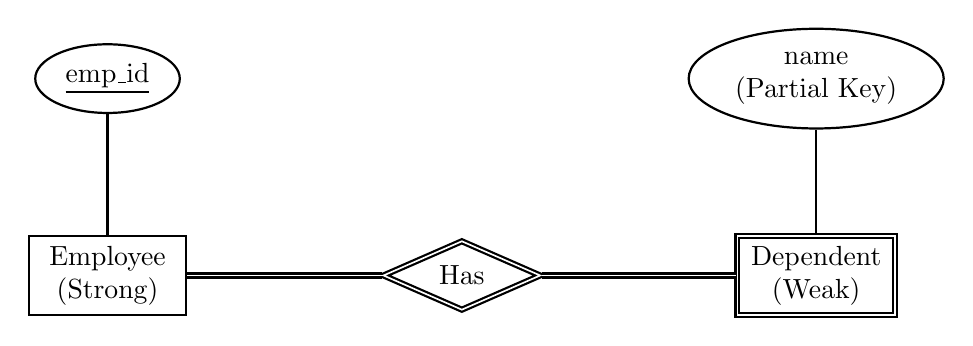
\begin{tikzpicture}[node distance=2.5cm, auto, thick]
    % Styles
    \tikzstyle{entity} = [draw, rectangle, minimum height=1cm, minimum width=2cm, align=center]
    \tikzstyle{weak entity} = [draw, rectangle, double, minimum height=1cm, minimum width=2cm, align=center]
    \tikzstyle{relationship} = [draw, diamond, aspect=2, minimum width=2cm, align=center]
    \tikzstyle{weak relationship} = [draw, diamond, double, aspect=2, minimum width=2cm, align=center]
    \tikzstyle{attribute} = [draw, ellipse, align=center]
    \tikzstyle{derived attribute} = [draw, ellipse, dashed, align=center]

    % Nodes
    \node [entity] (Emp) {Employee\\(Strong)};
    \node [weak relationship, right of=Emp, xshift=2cm] (Has) {Has};
    \node [weak entity, right of=Has, xshift=2cm] (Dep) {Dependent\\(Weak)};
    
    % Attributes
    \node [attribute, above of=Emp] (EmpID) {\underline{emp\_id}};
    \node [attribute, above of=Dep] (Name) {name\\(Partial Key)};
    
    % Connections
    \draw (EmpID) -- (Emp);
    \draw [double] (Emp) -- (Has);
    \draw [double] (Has) -- (Dep);
    \draw (Dep) -- (Name);
\end{tikzpicture}
\captionof{figure}{Strong vs Weak Entity}
\end{center}

\begin{center}
\captionof{table}{Weak vs Strong Entity}
\begin{tabulary}{\linewidth}{|L|L|L|}
\hline
\textbf{Aspect} & \textbf{Strong Entity} & \textbf{Weak Entity} \\ \hline
\textbf{Primary Key} & Has its own primary key & No primary key \\ \hline
\textbf{Existence} & Independent existence & Depends on strong entity \\ \hline
\textbf{Representation} & Single rectangle & Double rectangle \\ \hline
\textbf{Example} & Employee & Dependent of Employee \\ \hline
\end{tabulary}
\end{center}

\begin{itemize}
    \item \keyword{Partial Key}: Attribute that partially identifies weak entity
    \item \keyword{Identifying Relationship}: Connects weak entity to strong entity
    \item \keyword{Total Participation}: Weak entity must participate in relationship
\end{itemize}
\end{solutionbox}

\begin{mnemonicbox}
\mnemonic{Weak entities are DEPENDent}
\end{mnemonicbox}

\questionmarks{2(c)}{7}{Draw ER Diagram for University Management System}

\begin{solutionbox}
\begin{center}
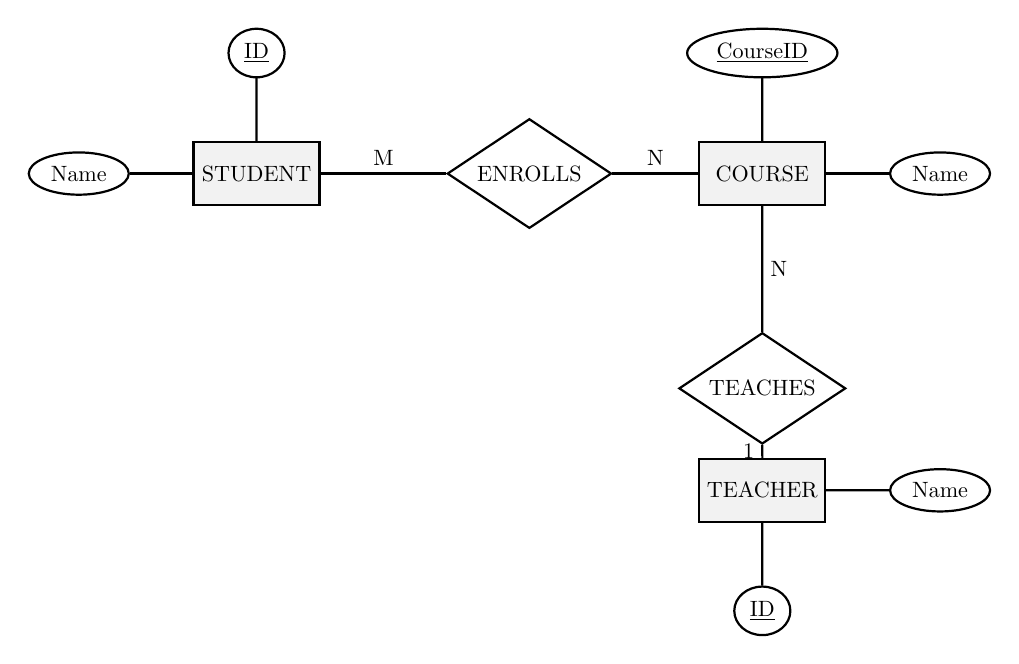
\begin{tikzpicture}[node distance=2cm, auto, thick, scale=0.8, transform shape]
    % Styles
    \tikzstyle{entity} = [draw, rectangle, minimum height=1cm, minimum width=2cm, align=center, fill=gray!10]
    \tikzstyle{relationship} = [draw, diamond, aspect=1.5, minimum width=2cm, align=center]
    \tikzstyle{attribute} = [draw, ellipse, align=center, node distance=1.5cm]

    % Entities
    \node [entity] (Std) {STUDENT};
    \node [entity, right=6cm of Std] (Crs) {COURSE};
    \node [entity, below=4cm of Crs] (Tch) {TEACHER};
    
    % Relationships
    \node [relationship, right=2cm of Std] (Enr) {ENROLLS};
    \node [relationship, below=2cm of Crs] (TchCrs) {TEACHES};
    
    % Attributes - Student
    \node [attribute, above=1cm of Std] (Sid) {\underline{ID}};
    \node [attribute, left=1cm of Std] (Sname) {Name};
    
    % Attributes - Course
    \node [attribute, above=1cm of Crs] (Cid) {\underline{CourseID}};
    \node [attribute, right=1cm of Crs] (Cname) {Name};
    
    % Attributes - Teacher
    \node [attribute, below=1cm of Tch] (Tid) {\underline{ID}};
    \node [attribute, right=1cm of Tch] (Tname) {Name};

    % Edges
    % Student - Enroll - Course
    \draw (Std) -- node[above]{M} (Enr);
    \draw (Enr) -- node[above]{N} (Crs);
    
    % Teacher - Teaches - Course
    \draw (Tch) -- node[left]{1} (TchCrs);
    \draw (TchCrs) -- node[right]{N} (Crs);
    
    % Connect Attributes
    \draw (Std) -- (Sid); \draw (Std) -- (Sname);
    \draw (Crs) -- (Cid); \draw (Crs) -- (Cname);
    \draw (Tch) -- (Tid); \draw (Tch) -- (Tname);
    
\end{tikzpicture}
\captionof{figure}{University ER Diagram}
\end{center}

\begin{center}
\captionof{table}{Entity Relationships}
\begin{tabulary}{\linewidth}{|L|C|L|}
\hline
\textbf{Relationship} & \textbf{Cardinality} & \textbf{Description} \\ \hline
\textbf{Student ENROLLS Course} & M:N & Many students can enroll in many courses \\ \hline
\textbf{Teacher TEACHES Course} & 1:N & One teacher teaches multiple courses \\ \hline
\textbf{Course HAS Enrollment} & 1:N & One course has multiple enrollments \\ \hline
\end{tabulary}
\end{center}

\begin{itemize}
    \item \keyword{Primary Entities}: Student, Course, Teacher
    \item \keyword{Associative Entity}: Enrollment (resolves M:N relationship)
    \item \keyword{Key Attributes}: All entities have unique identifier
\end{itemize}
\end{solutionbox}

\begin{mnemonicbox}
\mnemonic{University = Students Take Courses from Teachers}
\end{mnemonicbox}

\questionmarks{2(a) OR}{3}{Define Following Terms: 1. Primary Key 2. Foreign Key 3. Candidate Key}

\begin{solutionbox}
\begin{center}
\captionof{table}{Database Keys}
\begin{tabulary}{\linewidth}{|L|L|L|}
\hline
\textbf{Key Type} & \textbf{Definition} & \textbf{Example} \\ \hline
\textbf{Primary Key} & Unique identifier for each record & Student\_ID in Student table \\ \hline
\textbf{Foreign Key} & References primary key of another table & Student\_ID in Enrollment table \\ \hline
\textbf{Candidate Key} & Potential primary key attribute & Email, Phone in Student table \\ \hline
\end{tabulary}
\end{center}

\begin{itemize}
    \item \keyword{Primary Key}: Cannot be NULL and must be unique
    \item \keyword{Foreign Key}: Maintains referential integrity
    \item \keyword{Candidate Key}: Alternative unique identifiers
\end{itemize}
\end{solutionbox}

\begin{mnemonicbox}
\mnemonic{PFC - Primary Foreign Candidate}
\end{mnemonicbox}

\questionmarks{2(b) OR}{4}{Write a Short note on Generalization and Specialization}

\begin{solutionbox}
\textbf{Generalization}: Process of extracting common attributes from multiple entities to create a general entity.

\textbf{Specialization}: Process of defining subclasses of an entity based on distinguishing characteristics.

\begin{center}
\begin{tikzpicture}[node distance=1.5cm, auto]
    % Nodes
    \node [gtu block] (Per) {Person};
    
    \node [gtu state, below=1cm of Per] (ISA1) {IS-A};
    
    \node [gtu block, below left=1.5cm and 0.5cm of ISA1] (Std) {Student};
    \node [gtu block, below=1.5cm of ISA1] (Tch) {Teacher};
    \node [gtu block, below right=1.5cm and 0.5cm of ISA1] (Stf) {Staff};
    
    \node [gtu state, below=1cm of Std] (ISA2) {IS-A};
    
    \node [gtu block, below left=1.5cm and 0.2cm of ISA2] (UG) {Undergrad};
    \node [gtu block, below right=1.5cm and 0.2cm of ISA2] (PG) {Graduate};
    
    % Arrows
    \draw [gtu arrow] (Per) -- (ISA1);
    \draw [gtu arrow] (ISA1) -| (Std);
    \draw [gtu arrow] (ISA1) -- (Tch);
    \draw [gtu arrow] (ISA1) -| (Stf);
    
    \draw [gtu arrow] (Std) -- (ISA2);
    \draw [gtu arrow] (ISA2) -| (UG);
    \draw [gtu arrow] (ISA2) -| (PG);

    % Annotation
    \node [right=1cm of ISA1, align=left] {$\leftarrow$ Generalization (Up)\\ $\rightarrow$ Specialization (Down)};

\end{tikzpicture}
\captionof{figure}{Generalization and Specialization Hierarchy}
\end{center}

\begin{center}
\captionof{table}{Generalization vs Specialization}
\begin{tabulary}{\linewidth}{|L|L|L|}
\hline
\textbf{Aspect} & \textbf{Generalization} & \textbf{Specialization} \\ \hline
\textbf{Direction} & Bottom-up approach & Top-down approach \\ \hline
\textbf{Purpose} & Remove redundancy & Add specific attributes \\ \hline
\textbf{Result} & Superclass creation & Subclass creation \\ \hline
\end{tabulary}
\end{center}

\begin{itemize}
    \item \keyword{ISA Relationship}: "Is-A" relationship between superclass and subclass
    \item \keyword{Inheritance}: Subclasses inherit attributes from superclass
\end{itemize}
\end{solutionbox}

\begin{mnemonicbox}
\mnemonic{General goes UP, Special goes DOWN}
\end{mnemonicbox}

\questionmarks{2(c) OR}{7}{Explain different Relational Algebra operation with example}

\begin{solutionbox}
\begin{center}
\captionof{table}{Relational Algebra Operations}
\begin{tabulary}{\linewidth}{|L|C|L|L|}
\hline
\textbf{Operation} & \textbf{Symbol} & \textbf{Description} & \textbf{Example} \\ \hline
\textbf{Select} & $\sigma$ & Selects rows based on condition & $\sigma_{age>20}(Student)$ \\ \hline
\textbf{Project} & $\pi$ & Selects specific columns & $\pi_{name,age}(Student)$ \\ \hline
\textbf{Union} & $\cup$ & Combines two relations & $R \cup S$ \\ \hline
\textbf{Intersection} & $\cap$ & Common tuples from relations & $R \cap S$ \\ \hline
\textbf{Difference} & $-$ & Tuples in R but not in S & $R - S$ \\ \hline
\textbf{Join} & $\bowtie$ & Combines related tuples & $Student \bowtie Enrollment$ \\ \hline
\end{tabulary}
\end{center}

\textbf{Example Relations:}
Student: (ID=1, Name=John, Age=20) \\
Course: (CID=101, CName=DBMS, Credits=3)

\begin{itemize}
    \item \keyword{Selection}: $\sigma_{Age>18}(Student)$ returns students above 18
    \item \keyword{Projection}: $\pi_{Name}(Student)$ returns only names
    \item \keyword{Join}: $Student \bowtie Enrollment$ combines student and enrollment data
\end{itemize}
\end{solutionbox}

\begin{mnemonicbox}
\mnemonic{SPUDIJ - Select Project Union Difference Intersection Join}
\end{mnemonicbox}


\questionmarks{3(a)}{3}{List out Numeric Functions in SQL. Explain any Two}

\begin{solutionbox}
\begin{center}
\captionof{table}{SQL Numeric Functions}
\begin{tabulary}{\linewidth}{|L|L|L|}
\hline
\textbf{Function} & \textbf{Purpose} & \textbf{Example} \\ \hline
\textbf{ABS()} & Absolute value & ABS(-15) = 15 \\ \hline
\textbf{CEIL()} & Smallest integer $\ge$ value & CEIL(4.3) = 5 \\ \hline
\textbf{FLOOR()} & Largest integer $\le$ value & FLOOR(4.7) = 4 \\ \hline
\textbf{ROUND()} & Round to specified places & ROUND(15.76, 1) = 15.8 \\ \hline
\textbf{SQRT()} & Square root & SQRT(16) = 4 \\ \hline
\textbf{POWER()} & Raise to power & POWER(2, 3) = 8 \\ \hline
\end{tabulary}
\end{center}

\textbf{Detailed Examples:}

\begin{itemize}
    \item \keyword{ABS(number)}: Returns absolute value, removing negative sign
    \item \keyword{ROUND(number, decimal\_places)}: Rounds number to specified decimal places
\end{itemize}
\end{solutionbox}

\begin{mnemonicbox}
\mnemonic{Math functions make Numbers Nice}
\end{mnemonicbox}

\questionmarks{3(b)}{4}{Describe Having and Order by Clause with example}

\begin{solutionbox}
\keyword{HAVING Clause}: Used with GROUP BY to filter groups based on aggregate conditions.

\keyword{ORDER BY Clause}: Used to sort result set in ascending or descending order.

\begin{center}
\captionof{table}{HAVING vs WHERE}
\begin{tabulary}{\linewidth}{|L|L|L|}
\hline
\textbf{Aspect} & \textbf{WHERE} & \textbf{HAVING} \\ \hline
\textbf{Usage} & Filters individual rows & Filters grouped results \\ \hline
\textbf{With Aggregates} & Cannot use & Can use aggregate functions \\ \hline
\textbf{Position} & Before GROUP BY & After GROUP BY \\ \hline
\end{tabulary}
\end{center}

\textbf{Example:}

\begin{lstlisting}[language=SQL]
SELECT department, COUNT(*) as emp_count
FROM employees 
WHERE salary > 30000
GROUP BY department 
HAVING COUNT(*) > 5
ORDER BY emp_count DESC;
\end{lstlisting}

\begin{itemize}
    \item \keyword{WHERE}: Filters employees with salary > 30000
    \item \keyword{HAVING}: Shows only departments with more than 5 employees
    \item \keyword{ORDER BY}: Sorts by employee count in descending order
\end{itemize}
\end{solutionbox}

\begin{mnemonicbox}
\mnemonic{WHERE filters rows, HAVING filters groups, ORDER BY sorts results}
\end{mnemonicbox}

\questionmarks{3(c)}{7}{Perform the following Query on the table student having the fields Student\_ID, Stu\_Name, Stu\_Subject\_ID, Stu\_Marks, Stu\_Age in SQL}

\begin{solutionbox}
\textbf{1. Create student table:}
\begin{lstlisting}[language=SQL]
CREATE TABLE student (
    Student_ID INT PRIMARY KEY,
    Stu_Name VARCHAR(50),
    Stu_Subject_ID INT,
    Stu_Marks INT,
    Stu_Age INT
);
\end{lstlisting}

\textbf{2. Insert record in student table:}
\begin{lstlisting}[language=SQL]
INSERT INTO student VALUES 
(1, "John", 101, 85, 22),
(2, "Mary", 102, 90, 21);
\end{lstlisting}

\textbf{3. Find minimum and maximum marks:}
\begin{lstlisting}[language=SQL]
SELECT MIN(Stu_Marks) as Min_Marks, 
       MAX(Stu_Marks) as Max_Marks 
FROM student;
\end{lstlisting}

\textbf{4. Students with marks > 82 and age = 22:}
\begin{lstlisting}[language=SQL]
SELECT * FROM student 
WHERE Stu_Marks > 82 AND Stu_Age = 22;
\end{lstlisting}

\textbf{5. Students whose name begins with "m":}
\begin{lstlisting}[language=SQL]
SELECT * FROM student 
WHERE Stu_Name LIKE "m%";
\end{lstlisting}

\textbf{6. Find average marks:}
\begin{lstlisting}[language=SQL]
SELECT AVG(Stu_Marks) as Average_Marks 
FROM student;
\end{lstlisting}

\textbf{7. Add Stu\_address column:}
\begin{lstlisting}[language=SQL]
ALTER TABLE student 
ADD Stu_address VARCHAR(100);
\end{lstlisting}
\end{solutionbox}

\begin{mnemonicbox}
\mnemonic{CRUD + Analytics = Complete Database Operations}
\end{mnemonicbox}

\questionmarks{3(a) OR}{3}{Describe different date function in SQL with example}

\begin{solutionbox}
\begin{center}
\captionof{table}{SQL Date Functions}
\begin{tabulary}{\linewidth}{|L|L|L|}
\hline
\textbf{Function} & \textbf{Purpose} & \textbf{Example} \\ \hline
\textbf{SYSDATE} & Current system date & SYSDATE returns '2024-06-12' \\ \hline
\textbf{ADD\_MONTHS()} & Add months to date & ADD\_MONTHS('2024-01-15', 3) \\ \hline
\textbf{MONTHS\_BETWEEN()} & Months between dates & MONTHS\_BETWEEN('2024-06-12', '2024-01-12') \\ \hline
\textbf{LAST\_DAY()} & Last day of month & LAST\_DAY('2024-02-15') = '2024-02-29' \\ \hline
\textbf{NEXT\_DAY()} & Next occurrence of day & NEXT\_DAY('2024-06-12', 'FRIDAY') \\ \hline
\end{tabulary}
\end{center}

\textbf{Examples:}
\begin{itemize}
    \item \keyword{SYSDATE}: Returns current system date and time
    \item \keyword{ADD\_MONTHS}: Useful for calculating future dates like loan due dates
\end{itemize}
\end{solutionbox}

\begin{mnemonicbox}
\mnemonic{Date functions help with Time Management}
\end{mnemonicbox}

\questionmarks{3(b) OR}{4}{List out Constraints in SQL. Explain any two with example}

\begin{solutionbox}
\begin{center}
\captionof{table}{SQL Constraints}
\begin{tabulary}{\linewidth}{|L|L|L|}
\hline
\textbf{Constraint} & \textbf{Purpose} & \textbf{Example} \\ \hline
\textbf{PRIMARY KEY} & Unique identifier & Student\_ID INT PRIMARY KEY \\ \hline
\textbf{FOREIGN KEY} & References another table & REFERENCES Student(Student\_ID) \\ \hline
\textbf{NOT NULL} & Prevents null values & Name VARCHAR(50) NOT NULL \\ \hline
\textbf{UNIQUE} & Ensures uniqueness & Email VARCHAR(100) UNIQUE \\ \hline
\textbf{CHECK} & Validates data & Age INT CHECK (Age >= 18) \\ \hline
\textbf{DEFAULT} & Default value & Status VARCHAR(10) DEFAULT 'Active' \\ \hline
\end{tabulary}
\end{center}

\textbf{Detailed Examples:}

\textbf{PRIMARY KEY Constraint:}
\begin{lstlisting}[language=SQL]
CREATE TABLE Student (
    Student_ID INT PRIMARY KEY,
    Name VARCHAR(50)
);
\end{lstlisting}

\textbf{CHECK Constraint:}
\begin{lstlisting}[language=SQL]
CREATE TABLE Employee (
    Emp_ID INT,
    Salary INT CHECK (Salary > 0)
);
\end{lstlisting}

\begin{itemize}
    \item \keyword{PRIMARY KEY}: Ensures each record has unique identifier
    \item \keyword{CHECK}: Validates business rules during data entry
\end{itemize}
\end{solutionbox}

\begin{mnemonicbox}
\mnemonic{Constraints Control Data Quality}
\end{mnemonicbox}

\questionmarks{3(c) OR}{7}{Explain different types of joins with example in SQL}

\begin{solutionbox}
\begin{center}
\captionof{table}{Types of SQL Joins}
\begin{tabulary}{\linewidth}{|L|L|L|}
\hline
\textbf{Join Type} & \textbf{Description} & \textbf{Syntax} \\ \hline
\textbf{INNER JOIN} & Returns matching records from both tables & Table1 INNER JOIN Table2 ON condition \\ \hline
\textbf{LEFT JOIN} & All records from left table + matching from right & Table1 LEFT JOIN Table2 ON condition \\ \hline
\textbf{RIGHT JOIN} & All records from right table + matching from left & Table1 RIGHT JOIN Table2 ON condition \\ \hline
\textbf{FULL OUTER JOIN} & All records from both tables & Table1 FULL OUTER JOIN Table2 ON condition \\ \hline
\end{tabulary}
\end{center}

\textbf{Example Tables:}
Students: (ID=1, Name=John), (ID=2, Name=Mary) \\
Enrollments: (StudentID=1, Course=DBMS), (StudentID=3, Course=Java)

\textbf{INNER JOIN Example:}
\begin{lstlisting}[language=SQL]
SELECT s.Name, e.Course 
FROM Students s 
INNER JOIN Enrollments e ON s.ID = e.StudentID;
\end{lstlisting}
\textit{Result: Only John with DBMS course}

\textbf{LEFT JOIN Example:}
\begin{lstlisting}[language=SQL]
SELECT s.Name, e.Course 
FROM Students s 
LEFT JOIN Enrollments e ON s.ID = e.StudentID;
\end{lstlisting}
\textit{Result: John-DBMS, Mary-NULL}
\end{solutionbox}

\begin{mnemonicbox}
\mnemonic{JOIN connects Related Tables}
\end{mnemonicbox}


\questionmarks{4(a)}{3}{Give an example of Grant and Revoke command in SQL}

\begin{solutionbox}
\keyword{GRANT Command}: Provides specific privileges to users on database objects.

\keyword{REVOKE Command}: Removes previously granted privileges from users.

\begin{center}
\captionof{table}{Common Privileges}
\begin{tabulary}{\linewidth}{|L|L|L|}
\hline
\textbf{Privilege} & \textbf{Description} & \textbf{Example} \\ \hline
\textbf{SELECT} & Read data & GRANT SELECT ON Student TO user1 \\ \hline
\textbf{INSERT} & Add new records & GRANT INSERT ON Student TO user1 \\ \hline
\textbf{UPDATE} & Modify existing records & GRANT UPDATE ON Student TO user1 \\ \hline
\textbf{DELETE} & Remove records & GRANT DELETE ON Student TO user1 \\ \hline
\textbf{ALL} & All privileges & GRANT ALL ON Student TO user1 \\ \hline
\end{tabulary}
\end{center}

\textbf{Examples:}
\begin{lstlisting}[language=SQL]
-- Grant SELECT privilege
GRANT SELECT ON Student TO john;

-- Revoke INSERT privilege  
REVOKE INSERT ON Student FROM john;
\end{lstlisting}

\begin{itemize}
    \item \keyword{WITH GRANT OPTION}: Allows user to grant privileges to others
    \item \keyword{CASCADE}: Revokes privileges from all users who received them
\end{itemize}
\end{solutionbox}

\begin{mnemonicbox}
\mnemonic{GRANT gives rights, REVOKE removes rights}
\end{mnemonicbox}

\questionmarks{4(b)}{4}{Write a short note on SQL Views}

\begin{solutionbox}
\textbf{Definition}: A view is a virtual table based on the result of an SQL statement containing rows and columns like a real table.

\begin{center}
\captionof{table}{View Characteristics}
\begin{tabulary}{\linewidth}{|L|L|L|}
\hline
\textbf{Aspect} & \textbf{Description} & \textbf{Example} \\ \hline
\textbf{Virtual Table} & Does not store data physically & CREATE VIEW student\_view AS... \\ \hline
\textbf{Security} & Hides sensitive columns & Hide salary column from employees \\ \hline
\textbf{Simplification} & Simplifies complex queries & Join multiple tables in single view \\ \hline
\textbf{Data Independence} & Changes in base tables don't affect users & Modify table structure without affecting applications \\ \hline
\end{tabulary}
\end{center}

\textbf{Example:}
\begin{lstlisting}[language=SQL]
CREATE VIEW active_students AS
SELECT Student_ID, Name, Age 
FROM Student 
WHERE Status = 'Active';

-- Using the view
SELECT * FROM active_students;
\end{lstlisting}

\begin{itemize}
    \item \keyword{Security}: Restrict access to sensitive data
    \item \keyword{Simplicity}: Hide complex joins from end users
    \item \keyword{Consistency}: Standardized data access
\end{itemize}
\end{solutionbox}

\begin{mnemonicbox}
\mnemonic{Views are Virtual Windows to Data}
\end{mnemonicbox}

\questionmarks{4(c)}{7}{What is Normalization? Explain 2NF with example}

\begin{solutionbox}
\textbf{Normalization}: Process of organizing database to reduce redundancy and improve data integrity by dividing large tables into smaller related tables.

\textbf{2NF (Second Normal Form)}:
\begin{itemize}
    \item Must be in 1NF
    \item Remove partial functional dependencies
    \item Non-key attributes must depend on entire primary key
\end{itemize}

\textbf{Example - Unnormalized Table:}
\begin{center}
\begin{tabulary}{\linewidth}{|L|L|L|L|L|}
\hline
\textbf{Student\_ID} & \textbf{Course\_ID} & \textbf{Student\_Name} & \textbf{Course\_Name} & \textbf{Instructor} \\ \hline
101 & C1 & John & DBMS & Dr. Smith \\ \hline
101 & C2 & John & Java & Dr. Jones \\ \hline
102 & C1 & Mary & DBMS & Dr. Smith \\ \hline
\end{tabulary}
\end{center}

\textbf{Problems:}
\begin{itemize}
    \item Student\_Name depends only on Student\_ID (partial dependency)
    \item Course\_Name and Instructor depend only on Course\_ID
\end{itemize}

\textbf{After 2NF:}

\textbf{Student Table:}
\begin{center}
\begin{tabulary}{\linewidth}{|L|L|}
\hline
\textbf{Student\_ID} & \textbf{Student\_Name} \\ \hline
101 & John \\ \hline
102 & Mary \\ \hline
\end{tabulary}
\end{center}

\textbf{Course Table:}
\begin{center}
\begin{tabulary}{\linewidth}{|L|L|L|}
\hline
\textbf{Course\_ID} & \textbf{Course\_Name} & \textbf{Instructor} \\ \hline
C1 & DBMS & Dr. Smith \\ \hline
C2 & Java & Dr. Jones \\ \hline
\end{tabulary}
\end{center}

\textbf{Enrollment Table:}
\begin{center}
\begin{tabulary}{\linewidth}{|L|L|}
\hline
\textbf{Student\_ID} & \textbf{Course\_ID} \\ \hline
101 & C1 \\ \hline
101 & C2 \\ \hline
102 & C1 \\ \hline
\end{tabulary}
\end{center}

\begin{itemize}
    \item \keyword{Eliminates Redundancy}: Student names not repeated
    \item \keyword{Reduces Storage}: Less duplicate data
    \item \keyword{Improves Consistency}: Update student name in one place
\end{itemize}
\end{solutionbox}

\begin{mnemonicbox}
\mnemonic{2NF = No Partial Dependencies}
\end{mnemonicbox}

\questionmarks{4(a) OR}{3}{Give an example of Group By Clause in SQL}

\begin{solutionbox}
\textbf{GROUP BY Clause}: Groups rows with same values in specified columns and allows aggregate functions on each group.

\begin{center}
\captionof{table}{GROUP BY Usage}
\begin{tabulary}{\linewidth}{|L|L|L|}
\hline
\textbf{Purpose} & \textbf{Function} & \textbf{Example} \\ \hline
\textbf{Counting} & COUNT() & Count students per department \\ \hline
\textbf{Summing} & SUM() & Total salary per department \\ \hline
\textbf{Averaging} & AVG() & Average marks per course \\ \hline
\textbf{Finding Min/Max} & MIN()/MAX() & Highest salary per department \\ \hline
\end{tabulary}
\end{center}

\textbf{Example:}
\begin{lstlisting}[language=SQL]
SELECT Department, COUNT(*) as Total_Students, AVG(Marks) as Avg_Marks
FROM Student 
GROUP BY Department;
\end{lstlisting}

\textbf{Result:}
\begin{center}
\begin{tabulary}{\linewidth}{|L|L|L|}
\hline
\textbf{Department} & \textbf{Total\_Students} & \textbf{Avg\_Marks} \\ \hline
IT & 25 & 78.5 \\ \hline
CS & 30 & 82.1 \\ \hline
\end{tabulary}
\end{center}

\begin{itemize}
    \item \keyword{Groups}: Creates separate groups for each department
    \item \keyword{Aggregates}: Calculates count and average for each group
\end{itemize}
\end{solutionbox}

\begin{mnemonicbox}
\mnemonic{GROUP BY creates Summary Reports}
\end{mnemonicbox}

\questionmarks{4(b) OR}{4}{Describe Set Operators in SQL with example}

\begin{solutionbox}
\textbf{Set Operators}: Combine results from two or more SELECT statements.

\begin{center}
\captionof{table}{SQL Set Operators}
\begin{tabulary}{\linewidth}{|L|L|L|L|}
\hline
\textbf{Operator} & \textbf{Description} & \textbf{Requirement} & \textbf{Example} \\ \hline
\textbf{UNION} & Combines results, removes duplicates & Same column structure & SELECT name FROM students UNION SELECT name FROM teachers \\ \hline
\textbf{UNION ALL} & Combines results, keeps duplicates & Same column structure & SELECT name FROM students UNION ALL SELECT name FROM alumni \\ \hline
\textbf{INTERSECT} & Returns common records & Same column structure & SELECT course FROM current\_courses INTERSECT SELECT course FROM popular\_courses \\ \hline
\textbf{MINUS} & Records in first query but not second & Same column structure & SELECT student\_id FROM enrolled MINUS SELECT student\_id FROM graduated \\ \hline
\end{tabulary}
\end{center}

\textbf{Example:}
\begin{lstlisting}[language=SQL]
-- Students who are also teachers
SELECT name FROM students
INTERSECT
SELECT name FROM teachers;

-- All people in university
SELECT name, 'Student' as type FROM students
UNION
SELECT name, 'Teacher' as type FROM teachers;
\end{lstlisting}

\begin{itemize}
    \item \keyword{Column Count}: Must be same in all queries
    \item \keyword{Data Types}: Corresponding columns must have compatible types
    \item \keyword{Order}: ORDER BY can only be used at the end
\end{itemize}
\end{solutionbox}

\begin{mnemonicbox}
\mnemonic{Set operators Unite, Intersect, and Subtract data}
\end{mnemonicbox}

\questionmarks{4(c) OR}{7}{Justify the importance of Normalization. Explain 1NF with example}

\begin{solutionbox}
\textbf{Importance of Normalization:}
\begin{center}
\captionof{table}{Benefits of Normalization}
\begin{tabulary}{\linewidth}{|L|L|L|}
\hline
\textbf{Benefit} & \textbf{Description} & \textbf{Impact} \\ \hline
\textbf{Eliminates Redundancy} & Reduces duplicate data storage & Saves storage space \\ \hline
\textbf{Prevents Anomalies} & Avoids insertion, deletion, update problems & Maintains data consistency \\ \hline
\textbf{Improves Integrity} & Ensures data accuracy & Reliable information system \\ \hline
\textbf{Flexible Design} & Easy to modify and extend & Adaptable to business changes \\ \hline
\end{tabulary}
\end{center}

\textbf{1NF (First Normal Form)}:
\begin{itemize}
    \item Eliminate duplicate columns from same table
    \item Create separate tables for related data
    \item Each cell contains single value (atomic values)
\end{itemize}

\textbf{Example - Unnormalized Table:}
\begin{center}
\begin{tabulary}{\linewidth}{|L|L|L|}
\hline
\textbf{Student\_ID} & \textbf{Name} & \textbf{Subjects} \\ \hline
101 & John & Math, Science, English \\ \hline
102 & Mary & Science, History \\ \hline
\end{tabulary}
\end{center}

\textbf{Problems:}
\begin{itemize}
    \item Subjects column contains multiple values
    \item Difficult to query specific subjects
    \item Update anomalies when adding/removing subjects
\end{itemize}

\textbf{After 1NF:}

\textbf{Student Table:}
\begin{center}
\begin{tabulary}{\linewidth}{|L|L|}
\hline
\textbf{Student\_ID} & \textbf{Name} \\ \hline
101 & John \\ \hline
102 & Mary \\ \hline
\end{tabulary}
\end{center}

\textbf{Student\_Subject Table:}
\begin{center}
\begin{tabulary}{\linewidth}{|L|L|}
\hline
\textbf{Student\_ID} & \textbf{Subject} \\ \hline
101 & Math \\ \hline
101 & Science \\ \hline
101 & English \\ \hline
102 & Science \\ \hline
102 & History \\ \hline
\end{tabulary}
\end{center}

\begin{itemize}
    \item \keyword{Atomic Values}: Each cell contains single value
    \item \keyword{Flexible Queries}: Easy to find students studying specific subjects
    \item \keyword{Easy Updates}: Add/remove subjects without affecting other data
\end{itemize}
\end{solutionbox}

\begin{mnemonicbox}
\mnemonic{1NF = One value per cell, No repeating groups}
\end{mnemonicbox}

\questionmarks{5(a)}{3}{Explain Serializability in Transaction Management}

\begin{solutionbox}
\textbf{Serializability}: Property that ensures concurrent execution of transactions produces same result as some serial execution of those transactions.

\begin{center}
\captionof{table}{Types of Serializability}
\begin{tabulary}{\linewidth}{|L|L|L|}
\hline
\textbf{Type} & \textbf{Description} & \textbf{Method} \\ \hline
\textbf{Conflict Serializability} & Based on conflicting operations & Precedence graph \\ \hline
\textbf{View Serializability} & Based on read-write patterns & View equivalence \\ \hline
\end{tabulary}
\end{center}

\textbf{Example:}
Transaction T1: R(A), W(A), R(B), W(B) \\
Transaction T2: R(A), W(A), R(B), W(B)

\textbf{Serial Schedule:} T1 $\to$ T2 or T2 $\to$ T1 \\
\textbf{Concurrent Schedule:} Interleaved operations

\begin{itemize}
    \item \keyword{Conflict Operations}: Operations on same data item where at least one is write
    \item \keyword{Serializable Schedule}: Equivalent to some serial schedule
    \item \keyword{Non-serializable}: May lead to inconsistent database state
\end{itemize}
\end{solutionbox}

\begin{mnemonicbox}
\mnemonic{Serializability ensures Transaction Consistency}
\end{mnemonicbox}

\questionmarks{5(b)}{4}{Describe Partial Functional Dependency with example}

\begin{solutionbox}
\textbf{Partial Functional Dependency}: When a non-key attribute is functionally dependent on only part of a composite primary key.

\begin{center}
\captionof{table}{Functional Dependency Types}
\begin{tabulary}{\linewidth}{|L|L|L|}
\hline
\textbf{Type} & \textbf{Definition} & \textbf{Example} \\ \hline
\textbf{Full Dependency} & Depends on entire primary key & (Student\_ID, Course\_ID) $\to$ Grade \\ \hline
\textbf{Partial Dependency} & Depends on part of primary key & (Student\_ID, Course\_ID) $\to$ Student\_Name \\ \hline
\end{tabulary}
\end{center}

\textbf{Example:} \\
\textbf{Enrollment Table:} \\
Primary Key: (Student\_ID, Course\_ID)

\begin{center}
\begin{tabulary}{\linewidth}{|L|L|L|L|L|}
\hline
\textbf{Student\_ID} & \textbf{Course\_ID} & \textbf{Student\_Name} & \textbf{Course\_Name} & \textbf{Grade} \\ \hline
101 & C1 & John & DBMS & A \\ \hline
101 & C2 & John & Java & B \\ \hline
\end{tabulary}
\end{center}

\textbf{Partial Dependencies:}
\begin{itemize}
    \item Student\_ID $\to$ Student\_Name (Student\_Name depends only on Student\_ID)
    \item Course\_ID $\to$ Course\_Name (Course\_Name depends only on Course\_ID)
\end{itemize}

\textbf{Problems:}
\begin{itemize}
    \item \keyword{Update Anomaly}: Changing student name requires multiple updates
    \item \keyword{Insertion Anomaly}: Cannot add student without enrolling in course
    \item \keyword{Deletion Anomaly}: Deleting enrollment may lose student information
\end{itemize}

\textbf{Solution}: Normalize to 2NF by removing partial dependencies
\end{solutionbox}

\begin{mnemonicbox}
\mnemonic{Partial dependency = Part of key determines attribute}
\end{mnemonicbox}

\questionmarks{5(c)}{7}{Write a Short note on Locking Mechanism with example in Transaction Management}

\begin{solutionbox}
\textbf{Locking Mechanism}: Concurrency control technique that prevents simultaneous access to data items during transaction execution.

\begin{center}
\captionof{table}{Types of Locks}
\begin{tabulary}{\linewidth}{|L|L|L|}
\hline
\textbf{Lock Type} & \textbf{Description} & \textbf{Usage} \\ \hline
\textbf{Shared Lock (S)} & Multiple transactions can read & Read operations \\ \hline
\textbf{Exclusive Lock (X)} & Only one transaction can access & Write operations \\ \hline
\textbf{Intention Lock} & Indicates intent to lock at lower level & Hierarchical locking \\ \hline
\end{tabulary}
\end{center}

\textbf{Two-Phase Locking (2PL) Protocol:}
\begin{itemize}
    \item \textbf{Growing Phase}: Acquire locks, cannot release any lock
    \item \textbf{Shrinking Phase}: Release locks, cannot acquire new locks
\end{itemize}

\textbf{Example:}
\begin{lstlisting}
Transaction T1: Read(A), Write(A), Read(B), Write(B)
Transaction T2: Read(A), Write(A), Read(C), Write(C)

T1: S-lock(A), Read(A), X-lock(A), Write(A), S-lock(B), 
    Read(B), X-lock(B), Write(B), Unlock(A), Unlock(B)

T2: Wait for A, S-lock(A), Read(A), X-lock(A), Write(A), 
    S-lock(C), Read(C), X-lock(C), Write(C), Unlock(A), Unlock(C)
\end{lstlisting}

\textbf{Lock Compatibility Matrix:}
\begin{center}
\begin{tabulary}{\linewidth}{|L|L|L|}
\hline
\textbf{Current/Requested} & \textbf{S} & \textbf{X} \\ \hline
\textbf{S} & \checkmark & \xmark \\ \hline
\textbf{X} & \xmark & \xmark \\ \hline
\end{tabulary}
\end{center}

\begin{itemize}
    \item \keyword{Deadlock}: Two transactions waiting for each other's locks
    \item \keyword{Starvation}: Transaction waits indefinitely for lock
\end{itemize}

\textbf{Solutions:}
\begin{itemize}
    \item \keyword{Deadlock Detection}: Use wait-for graph
    \item \keyword{Deadlock Prevention}: Timestamp-based protocols
\end{itemize}
\end{solutionbox}

\begin{mnemonicbox}
\mnemonic{Locking prevents Concurrent Conflicts}
\end{mnemonicbox}

\questionmarks{5(a) OR}{3}{Explain Deadlock in Transaction Management}

\begin{solutionbox}
\textbf{Deadlock}: Situation where two or more transactions are waiting indefinitely for each other to release locks, creating a circular wait condition.

\begin{center}
\captionof{table}{Deadlock Components}
\begin{tabulary}{\linewidth}{|L|L|L|}
\hline
\textbf{Component} & \textbf{Description} & \textbf{Example} \\ \hline
\textbf{Mutual Exclusion} & Resources cannot be shared & Exclusive locks \\ \hline
\textbf{Hold and Wait} & Process holds resources while waiting & T1 holds A, waits for B \\ \hline
\textbf{No Preemption} & Resources cannot be forcibly taken & Locks cannot be revoked \\ \hline
\textbf{Circular Wait} & Circular chain of waiting processes & T1$\to$T2$\to$T1 \\ \hline
\end{tabulary}
\end{center}

\textbf{Example:}
\begin{lstlisting}
Transaction T1: Lock(A), Lock(B)
Transaction T2: Lock(B), Lock(A)

Time 1: T1 gets Lock(A)
Time 2: T2 gets Lock(B) 
Time 3: T1 waits for Lock(B) - held by T2
Time 4: T2 waits for Lock(A) - held by T1
Result: DEADLOCK!
\end{lstlisting}

\begin{itemize}
    \item \keyword{Detection}: Use wait-for graph to identify cycles
    \item \keyword{Prevention}: Use timestamp ordering or wound-wait protocols
\end{itemize}
\end{solutionbox}

\begin{mnemonicbox}
\mnemonic{Deadlock = Circular Waiting for Resources}
\end{mnemonicbox}

\questionmarks{5(b) OR}{4}{Describe Full Functional Dependency with example}

\begin{solutionbox}
\textbf{Full Functional Dependency}: A non-key attribute is functionally dependent on the entire primary key (not just part of it).

\begin{center}
\captionof{table}{Dependency Comparison}
\begin{tabulary}{\linewidth}{|L|L|L|}
\hline
\textbf{Type} & \textbf{Definition} & \textbf{Example} \\ \hline
\textbf{Full Dependency} & Depends on complete primary key & (Student\_ID, Course\_ID) $\to$ Grade \\ \hline
\textbf{Partial Dependency} & Depends on part of primary key & (Student\_ID, Course\_ID) $\to$ Student\_Name \\ \hline
\end{tabulary}
\end{center}

\textbf{Example:} \\
\textbf{Enrollment Table:} \\
Primary Key: (Student\_ID, Course\_ID)

\begin{center}
\begin{tabulary}{\linewidth}{|L|L|L|L|}
\hline
\textbf{Student\_ID} & \textbf{Course\_ID} & \textbf{Grade} & \textbf{Hours} \\ \hline
101 & C1 & A & 4 \\ \hline
101 & C2 & B & 3 \\ \hline
102 & C1 & B & 4 \\ \hline
\end{tabulary}
\end{center}

\textbf{Full Functional Dependencies:}
\begin{itemize}
    \item (Student\_ID, Course\_ID) $\to$ Grade \checkmark
    \item (Student\_ID, Course\_ID) $\to$ Hours \checkmark
\end{itemize}

\textbf{Explanation:}
\begin{itemize}
    \item \keyword{Grade} depends on both Student\_ID AND Course\_ID (specific student in specific course)
    \item \keyword{Hours} also depends on both (student's hours in specific course)
    \item Cannot determine Grade from Student\_ID alone
    \item Cannot determine Grade from Course\_ID alone
\end{itemize}

\textbf{Benefits:}
\begin{itemize}
    \item \keyword{No Update Anomalies}: Changes affect only relevant records
    \item \keyword{Proper Normalization}: Supports 2NF requirements
    \item \keyword{Data Integrity}: Ensures accurate relationships
\end{itemize}
\end{solutionbox}

\begin{mnemonicbox}
\mnemonic{Full dependency needs Complete Key}
\end{mnemonicbox}

\questionmarks{5(c) OR}{7}{Explain ACID Properties of Transaction with example}

\begin{solutionbox}
\textbf{ACID Properties}: Four fundamental properties that guarantee database transaction reliability.

\begin{center}
\captionof{table}{ACID Properties}
\begin{tabulary}{\linewidth}{|L|L|L|}
\hline
\textbf{Property} & \textbf{Description} & \textbf{Example} \\ \hline
\textbf{Atomicity} & All or nothing execution & Bank transfer: both debit and credit must happen \\ \hline
\textbf{Consistency} & Database remains in valid state & Account balance cannot be negative \\ \hline
\textbf{Isolation} & Transactions don't interfere & Concurrent transactions appear sequential \\ \hline
\textbf{Durability} & Committed changes are permanent & Data survives system crashes \\ \hline
\end{tabulary}
\end{center}

\textbf{Detailed Examples:}

\textbf{Atomicity Example:}
\begin{lstlisting}[language=SQL]
BEGIN TRANSACTION;
UPDATE Account SET Balance = Balance - 1000 WHERE AccNo = 'A001';
UPDATE Account SET Balance = Balance + 1000 WHERE AccNo = 'A002';
COMMIT;
\end{lstlisting}
\textit{If either update fails, entire transaction is rolled back}

\textbf{Consistency Example:}
\begin{lstlisting}[language=SQL]
-- Before: A001 = 5000, A002 = 3000, Total = 8000
-- Transfer 1000 from A001 to A002
-- After: A001 = 4000, A002 = 4000, Total = 8000
-- Total money in system remains constant
\end{lstlisting}

\textbf{Isolation Example:}
\begin{lstlisting}
T1: Read(A=100), A=A+50, Write(A=150)
T2: Read(A=100), A=A*2, Write(A=200)
Serial Result: A=300 or A=250
Isolated execution must produce one of these results
\end{lstlisting}

\textbf{Durability Example:}
\begin{lstlisting}
After COMMIT is executed, even if system crashes,
the transferred amount remains in destination account
\end{lstlisting}

\textbf{Implementation:}
\begin{itemize}
    \item \keyword{Atomicity}: Using transaction logs and rollback
    \item \keyword{Consistency}: Using constraints and triggers
    \item \keyword{Isolation}: Using locking mechanisms
    \item \keyword{Durability}: Using write-ahead logging
\end{itemize}
\end{solutionbox}

\begin{mnemonicbox}
\mnemonic{ACID keeps Transactions Reliable}
\end{mnemonicbox}

\end{document}
